\documentclass[journal]{IEEEtran}

% *** CITATION PACKAGES ***
\usepackage{cite}

% *** GRAPHICS RELATED PACKAGES ***
\usepackage{graphicx}
\graphicspath{{figures/}{./figures/}{../figures/}}
\DeclareGraphicsExtensions{.pdf,.jpeg,.png,.eps}

% *** MATH PACKAGES ***
\usepackage{amsmath,amssymb,amsfonts}

% *** TABLE PACKAGES ***
\usepackage{booktabs}
\usepackage{multirow}
\usepackage{array}

% *** URL AND HYPERLINK PACKAGES ***
\usepackage{url}
\providecommand{\doi}[1]{\url{https://doi.org/#1}}

% *** TYPOGRAPHY ***
\usepackage{microtype}

\begin{document}

\title{MCG-TTA: Multi-Scale Consistency-Guided Test-Time Augmentation for Brain Tumor MRI Diagnosis}

\author{Anonymous~Authors%
\thanks{Manuscript draft submitted for peer review. Code, configs, and pre-trained weights will be made publicly available upon publication.}}

\markboth{IEEE Transactions on Medical Imaging,~Draft~Manuscript,~October~2026}%
{Anonymous Authors: MCG-TTA: Multi-Scale Consistency-Guided Test-Time Augmentation}

\maketitle

\begin{abstract}
Clinical image-analysis systems operate under strict limits on memory, latency, and the transmission of sensitive patient data. State-of-the-art models, however, continue to grow in size and compute, a trend that fits resource-constrained deployment poorly.
This study systematically evaluates deep learning models with fewer than one million parameters on small-to-medium-sized datasets for image classification and detection, focusing on efficiency and cross-dataset generalization. Results show that on saturated classification benchmarks, compact models can achieve performance statistically comparable to models an order of magnitude larger. The best model attains 98.3\% accuracy at 0.36 GFLOPs, running six times faster with less than a one-percentage-point accuracy difference. However, a performance gap remains on more challenging cross-dataset tasks, with errors concentrated in low-confidence predictions sensitive to input perturbations. The most efficient architecture, which uses parallel atrous convolution branches to capture multi-scale features, is particularly vulnerable to scale-sensitive inputs.
To address this limitation, we propose \textbf{MCG-TTA}, an architecture-informed inference strategy designed to improve robustness while limiting computational overhead. MCG-TTA improves slice-level F1 by up to 1.8 percentage points at approximately 1.9$\times$ the baseline latency, while retaining a model size of 0.91 million parameters. These findings suggest that, for resource-constrained clinical applications, uncertainty-aware inference can recover residual accuracy more efficiently than increasing model complexity.
\end{abstract}
\begin{IEEEkeywords}
Brain MRI, convolutional neural networks, compact neural networks, test-time augmentation, glioma grading, edge inference
\end{IEEEkeywords}

\IEEEpeerreviewmaketitle

\section{Introduction}
Medical image classification has benefited substantially from deeper architectures and transfer learning \cite{litjens2017,tajbakhsh2016}, but a model suitable for a retrospective benchmark is not necessarily suitable for local inference. A clinical workstation or resource-limited site must accommodate finite memory, predictable processing time, and restrictions on transmitting sensitive images \cite{kaissis2021}. These constraints make the conventional response to an accuracy shortfall---a larger backbone or a more expensive ensemble---particularly costly. The pertinent question is how far a compact network's reduced compute remains useful as the imaging task becomes harder.

Brain MRI makes this question concrete. A four-category collection of individual images distinguishes glioma, meningioma, pituitary tumor, and no tumor \cite{nickparvar}; high performance on this collection can conceal the difficulty of grading glioma across patients and imaging sequences \cite{menze2015}. The latter task changes both the label space and the acquisition setting. Consequently, accuracy on the first benchmark must not be interpreted as an estimate of grading performance on the second. Nor does a correct slice prediction, by itself, establish a correct patient-level decision. The distinction is most consequential when a minority grade is missed despite apparently favorable aggregate accuracy.

Recent work on sub-million-parameter vision networks directs limited capacity toward diverse spatial features rather than merely shrinking established backbones \cite{kyrkou2026}. Its LS-Net architecture uses parallel atrous depthwise paths to aggregate context at different receptive fields. For MRI, this design suggests an opportunity and a potential weakness: a compact model may be fast enough for local inference while predictions for borderline slices remain sensitive to changes in apparent scale. Instead of adding parameters to every prediction, one can allocate extra inference only to those predictions for which additional views may be informative. Sensitivity to an input transform is an observed operational criterion for a gate, not proof that a particular convolution branch causes an individual error.

This work asks two connected questions. First, how far can strictly sub-1M networks approach fine-tuned, multi-million-parameter backbones on a curated brain MRI classification benchmark, and does that relationship persist on a separate glioma-grading task? Second, can architecture-informed selective inference recover some of the grading gap without expanding the learned model? We compare compact scratch-trained architectures with fine-tuned larger backbones, examine class-level errors and paired significance tests, and study patient-level as well as slice-level outcomes. We then introduce multi-scale consistency-guided test-time augmentation (MCG-TTA) for LS-Net: a confidence gate selects uncertain slices, two scale views test prediction consistency, and only disagreements receive the remaining views.

Our contributions are:
\begin{enumerate}
\item We benchmark sub-1M-parameter architectures for efficiency and cross-task generalization, spanning four-class brain tumor classification and BraTS glioma grading, and quantify where compact models lose ground to larger backbones.
\item We propose \textbf{MCG-TTA}, a parameter-free, architecture-informed test-time augmentation strategy that improves slice-level F1 by up to 1.8 percentage points at roughly 1.9$\times$ baseline latency.
\end{enumerate}

\section{Related Work}
\subsection{Compact Vision Models}
Residual networks \cite{he2016}, VGG \cite{simonyan2015}, EfficientNet \cite{tan2019}, and MobileNetV2 \cite{sandler2018} represent different routes to high accuracy or reduced computation. The parameter count alone, however, does not determine batch-one CPU latency: depthwise operations, feature-map size, and implementation details also affect execution \cite{kyrkou2026}. Although lightweight vision transformers have narrowed the gap with CNNs on general benchmarks \cite{mehta2022}, they tend to underperform convolutional architectures in data-constrained, sub-1M-parameter settings \cite{kyrkou2026}. For medical images, fine-tuned pretrained backbones provide strong reference points \cite{tajbakhsh2016}, but a comparison restricted to similarly large pretrained models cannot establish what is lost by imposing a much tighter memory budget. We therefore contrast pretrained, fine-tuned backbones with scratch-trained compact counterparts rather than treating their training regimes as equivalent.

Kyrkou's LS-Net was designed for the sub-1M vision regime using multi-path atrous convolutions \cite{kyrkou2026}. Parallel depthwise paths with distinct dilation factors enlarge the set of spatial contexts represented without requiring a proportionate increase in learned parameters. In the present work, LS-Net serves as an adapted architectural baseline; our contribution is the inference strategy, not the backbone. The new question is whether such an architecture remains useful across two MRI tasks and whether its errors can be selectively addressed at inference time. A compact MPAC-ResNet variant helps separate the value of parallel atrous processing from the broader architectural choices of LS-Net.

\subsection{Distribution Shift and Test-Time Augmentation}
A high score on a balanced collection of two-dimensional images cannot establish robustness to different MR sequences, clinical labels, or subject composition \cite{guan2022}. In BraTS, HGG and LGG are grades rather than the tumor-type labels of the first benchmark \cite{menze2015}. We therefore report task-specific results and do not present the two test sets as interchangeable estimates of one distribution. Splitting by subject avoids putting different slices from the same patient in both training and test sets, a leakage mechanism documented in brain MRI classification \cite{yagis2021}. Patient-level aggregation also prevents repeated slices of one subject from being mistaken for independent clinical cases.

Test-time augmentation averages predictions from transformed versions of the same input, an approach studied in medical imaging as well as general image classification \cite{wang2019,moshkov2020,shanmugam2021}. Recent generative approaches use diffusion models to produce domain-aware augmented views at test time \cite{ma2026}, but their computational overhead is substantially higher than deterministic transforms. Unconditional use improves coverage at a compute cost on every slice, but can also overturn correct predictions \cite{shanmugam2021}; confidence gating spends compute on a smaller subset, but confidence alone cannot identify which transform is informative. A softmax score is also not necessarily a calibrated estimate of correctness \cite{guo2017}. Our method couples a low-confidence gate to a pair of scale probes that are motivated by LS-Net's multi-scale feature paths. Disagreement with the original prediction determines whether to acquire the remaining views. This is an inference-time intervention, not a change to training, calibration, or network weights.

\section{Methodology}
\subsection{Datasets and Evaluation}
The in-domain experiment uses the Nickparvar brain tumor MRI collection \cite{nickparvar} with the four categories glioma, meningioma, no tumor, and pituitary tumor. Duplicate and invalid images are removed before the stratified training, validation, and test split; the reported held-out test set contains 1,052 images and is approximately balanced. The configured split proportions are 70/15/15. Images are resized to $224\times224$ and normalized. Training-time transforms include rotation, horizontal reflection, scale changes, intensity variation, and elastic deformation. The primary outcomes are image accuracy and macro F1; specificity and AUC provide complementary class-discrimination summaries. The no-tumor label permits an image-level tumor-presence decision, but no spatial lesion detector is evaluated.

The second experiment uses BraTS 2020 \cite{menze2015,baid2021} to classify high-grade (HGG) versus low-grade (LGG) glioma from axial slices. FLAIR, contrast-enhanced T1, and T2 sequences are stacked as three input channels after per-volume intensity normalization. Tumor-containing axial slices are selected using segmentation masks during dataset construction, with a cap per subject, and are then resized for classification. Grade labels attach to subjects, not independently diagnosed slices. Subjects, rather than slices, are assigned to disjoint stratified splits before slice-level evaluation to avoid within-subject leakage \cite{yagis2021}. The test comparison covers 1,400 slices from 56 subjects, with an approximately 4:1 class imbalance. For patient-level inference, probabilities across a patient's evaluated slices are averaged and the largest mean determines the grade. Mask-based slice selection restricts this study to preselected, tumor-containing slices.

\begin{figure*}[t]
\centering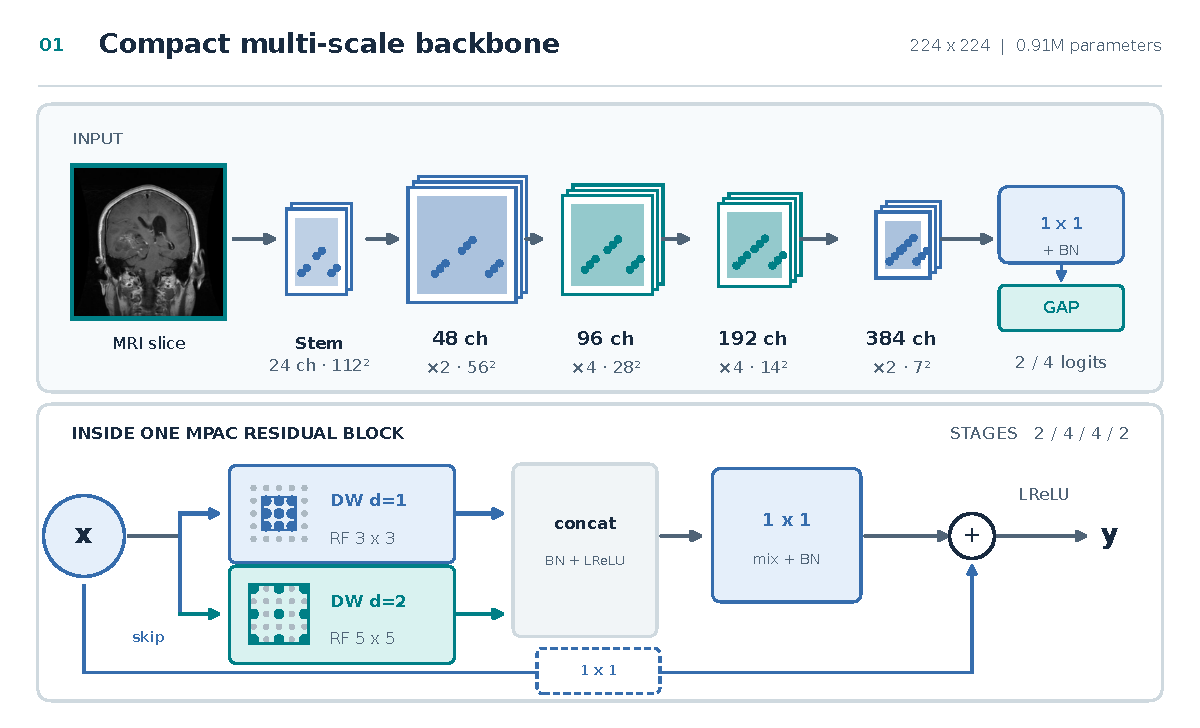
\includegraphics[width=0.88\textwidth]{figures/lsnet_architecture.pdf}
\caption{LS-Net backbone used for both tasks. The stem and four residual MPAC stages reduce spatial resolution while increasing channel width; the task-specific $1\times1$ head maps features to two or four logits. The enlarged block shows the parallel depthwise atrous paths (dilations 1 and 2), channel mixing, and residual connection.}\label{fig:lsnet-architecture}
\end{figure*}

\subsection{Models and Training}
We study fine-tuned ResNet-50, ResNet-18, VGG-16, EfficientNet-B0, and MobileNetV2 alongside compact scratch-trained LS-Net, ResNet-Tiny, MPAC-ResNet-Tiny, EfficientNet-Tiny, and MobileNet-Tiny. The hybrid MPAC-ResNet is included as a separate, above-1M comparison and is not counted as satisfying the strict sub-1M constraint. The compact LS-Net implementation adapts the architecture of Kyrkou \cite{kyrkou2026} with a strided stem and four stages built from residual multi-path atrous blocks (Fig.~\ref{fig:lsnet-architecture}). Each block computes parallel depthwise $3\times3$ convolutions with dilation factors $1$ and $2$, concatenates their outputs, mixes channels with a pointwise convolution, and adds a residual projection when required. The model has 0.91M parameters in both experiments; the different output heads implement the appropriate task labels.

The shared configuration uses $224\times224$ inputs, batch size 32, AdamW with cosine learning-rate scheduling, and validation macro F1 for checkpoint selection. Class weights are enabled for the imbalanced BraTS task. Multi-seed summaries use seeds 42, 123, and 456, except the TTA ablation, which uses the first two. Because pretrained backbones and scratch-trained compact models lack matched initialization, the results establish attainable performance under the specified protocols rather than isolating parameter count as the only causal factor. The four-class table reports sample standard deviations across three seeds, while the two-seed TTA ablation has different dispersion conventions. Pairwise McNemar tests \cite{mcnemar1947} use matched predictions on the 1,052-image four-class test set, with a nominal $0.05$ significance level; failure to reject a difference is not a formal equivalence test.

\subsection{Multi-Scale Consistency-Guided Test-Time Augmentation}
Let $p_0(y\mid x)$ be the LS-Net softmax probability for the unmodified slice $x$, $\hat y_0=\arg\max_y p_0(y\mid x)$, and $c(x)=\max_y p_0(y\mid x)$. A slice passes through the confidence gate when $c(x)<\tau$. Non-gated slices retain $p_0$ without another network call. Gated slices receive deterministic $0.9\times$ and $1.1\times$ scale views (Fig.~\ref{fig:mcg-tta}), yielding $p_-$ and $p_+$. If both scale-view argmax labels equal $\hat y_0$, the returned probability is the mean of the identity and the two scale-view probabilities. Otherwise, the slice escalates to a six-view mean over the identity, both scale views, horizontal flip, and positive and negative rotations. The rotations follow the configured $15^\circ$ augmentation limit. The averaged probability supplies the final slice decision.

Writing $G=\mathbb{1}[c(x)<\tau]$ and $D=\mathbb{1}[\arg\max p_-\ne\hat y_0\ \mathrm{or}\ \arg\max p_+\ne\hat y_0]$, the number of additional model evaluations per slice is $2G+3GD$. The modelled mean latency is therefore $t_0[1+2\Pr(G)+3\Pr(GD)]$, where $t_0$ is the single-forward baseline under the TTA profiling protocol. This formula accounts for conditional network calls but not transformation overhead or end-to-end clinical workflow time. The two probes are informed by the use of multiple dilation scales; neither dilation nor zoom is asserted to be physically equivalent, and the method should be interpreted as an empirical scale-consistency test. Unlike retraining or ensembling independent models, it adds no learned parameters.

\subsection{Efficiency Metrics}
Parameters, floating-point operations per image, model footprint, and batch-one CPU inference time characterize deployment cost. Throughput is the reciprocal of single-image latency under the reported profiling setup. Efficiency was profiled with single-thread PyTorch 2.x inference on an Intel Core CPU using 50 warm-up and 200 timed iterations. Separately, the TTA ablation reports \emph{modelled} latency from a baseline single-forward estimate of 5.60 ms, a different timing series from the 11.30 ms CPU profile. Multiplying the separately profiled LS-Net latency by the TTA relative factor yields an illustrative effective CPU estimate only. We keep the timing series separate throughout.

\input{sections/04_experiments}
\section{Discussion}
The two tasks expose why compactness cannot be judged by a single headline score. On the balanced four-class benchmark, multiple compact models reach approximately 98\% accuracy, and paired McNemar tests do not resolve a difference between LS-Net and ResNet-50 for the reported seeds. This supports a useful operating point at 0.91M parameters and 0.36 GFLOPs without implying that all compact models are equivalent or that added capacity has no benefit. On BraTS, the strongest model evaluated is instead VGG-16, and the gap between its 89.31\% slice F1 and LS-Net's 82.02\% is 7.29 points. Transformer-based architectures such as Swin UNETR \cite{hatamizadeh2022} have since become competitive baselines for brain tumor analysis, but their multi-million-parameter designs make it worth measuring what compact CNNs can and cannot achieve at the edge. Different model rankings and class-level outcomes warn against using performance on a curated tumor-type benchmark as a proxy for HGG/LGG grading.

MCG-TTA changes the allocation of compute rather than the representational capacity of the learned classifier. It uses identity confidence to select a subset of slices and scale-view disagreement to decide whether all views are needed. The ablation makes clear that the value of the architecture-informed rule is conditional: a flip-based strategy slightly surpasses it on mean slice F1, while full confidence-gated augmentation approaches its F1 at higher modelled cost. Its more favorable LGG preservation relative to some alternative gates is an observed result on 24 pooled LGG patient decisions. The residual miss rate, reduced patient F1 versus the unaugmented model, and absence of independent clinical validation rule out autonomous diagnostic claims.

Several limitations constrain the interpretation. BraTS grading is a separate training-and-testing problem, so these results measure robustness of model choice across tasks rather than invariance of one learned decision rule. Mask-guided selection of tumor-containing slices assumes information that may be unavailable when screening a new scan. Slice-level observations are correlated within subjects, and the minority-class patient count is small. Our analysis did not record what fraction of errors is low-confidence or scale-unstable, so this relationship remains a motivating qualitative observation rather than a measured prevalence or causal attribution. The four-class table reports three seeds, but the detailed TTA ablation reports two; claims about the TTA gain should be limited to that ablation. McNemar's non-significant results are not equivalence proofs, and adaptive latency is modelled from forward-pass counts rather than directly measured on a clinical device. Finally, the present study does not measure lesion localization, segmentation, cloud privacy outcomes, calibration, or radiologist performance.

These boundaries point to concrete next evaluations: prospective subject-level grading, direct end-to-end latency on target hardware, uncertainty calibration, and studies in which slice selection does not rely on segmentation masks. They would determine whether the present efficiency and slice-level gains translate into a reliable patient workflow.

\section{Conclusion}
A strict sub-million-parameter budget does not preclude strong brain MRI image classification: LS-Net obtains 98.29\% four-class accuracy with 0.36 GFLOPs and roughly sixfold lower CPU latency than ResNet-50 for a 0.85-point accuracy difference. The separate BraTS experiment exposes a substantial grading gap and prevents treating benchmark saturation as evidence of general clinical readiness. With the learned model fixed at 0.91M parameters, MCG-TTA raises mean slice F1 from 82.02\% to 83.45\% across the reported two-seed ablation, with a maximum 1.83-point gain, at a modelled 1.92$\times$ base latency. It retains the baseline's 20/24 pooled LGG patient detections but does not improve baseline patient F1. The central lesson is therefore a qualified one: selectively spending inference compute on uncertain, scale-inconsistent inputs can recover some residual slice-level performance without increasing model size, while patient-level utility and clinical deployment require additional validation.

\begin{thebibliography}{21}
\bibitem{baid2021} Baid, U., et al.: The RSNA-ASNR-MICCAI BraTS 2021 benchmark on brain tumor segmentation and radiogenomic classification. arXiv preprint arXiv:2107.02314 (2021)
\bibitem{guan2022} Guan, H., Liu, M.: Domain adaptation for medical image analysis: A survey. IEEE Transactions on Biomedical Engineering \textbf{69}(3), 1173--1185 (2022)
\bibitem{guo2017} Guo, C., Pleiss, G., Sun, Y., Weinberger, K.Q.: On calibration of modern neural networks. In: Proceedings of the 34th International Conference on Machine Learning, pp. 1321--1330 (2017)
\bibitem{hatamizadeh2022} Hatamizadeh, A., Nath, V., Tang, Y., Yang, D., Roth, H.R., Xu, D.: Swin UNETR: Swin transformers for semantic segmentation of brain tumors in MRI images. In: Brainlesion: Glioma, Multiple Sclerosis, Stroke and Traumatic Brain Injuries. LNCS, vol. 12962, pp. 272--284. Springer (2022)
\bibitem{he2016} He, K., Zhang, X., Ren, S., Sun, J.: Deep residual learning for image recognition. In: Proceedings of the IEEE Conference on Computer Vision and Pattern Recognition, pp. 770--778 (2016)
\bibitem{kaissis2021} Kaissis, G., et al.: End-to-end privacy preserving deep learning on multi-institutional medical imaging. Nature Machine Intelligence \textbf{3}, 473--484 (2021). \doi{10.1038/s42256-021-00337-8}
\bibitem{kyrkou2026} Kyrkou, C.: Rethinking compact ($<1$M) vision models: Balancing accuracy and speed through multi-path atrous convolutions. In: Proceedings of the IEEE/CVF Conference on Computer Vision and Pattern Recognition (CVPR) Findings, pp. 2710--2720 (2026)
\bibitem{litjens2017} Litjens, G., et al.: A survey on deep learning in medical image analysis. Medical Image Analysis \textbf{42}, 60--88 (2017). \doi{10.1016/j.media.2017.07.005}
\bibitem{ma2026} Ma, X., Tao, Y., et al.: Test-time generative augmentation for medical image segmentation. Medical Image Analysis \textbf{109}, 103902 (2026)
\bibitem{mcnemar1947} McNemar, Q.: Note on the sampling error of the difference between correlated proportions or percentages. Psychometrika \textbf{12}(2), 153--157 (1947). \doi{10.1007/BF02295996}
\bibitem{mehta2022} Mehta, S., Rastegari, M.: MobileViT: Light-weight, general-purpose, and mobile-friendly vision transformer. In: International Conference on Learning Representations (2022)
\bibitem{menze2015} Menze, B.H., et al.: The multimodal brain tumor image segmentation benchmark (BRATS). IEEE Transactions on Medical Imaging \textbf{34}(10), 1993--2024 (2015)
\bibitem{moshkov2020} Moshkov, N., Mathe, B., Kertesz-Farkas, A., Hollandi, R., Horvath, P.: Test-time augmentation for deep learning-based cell segmentation on microscopy images. Scientific Reports \textbf{10}, 5068 (2020). \doi{10.1038/s41598-020-61808-3}
\bibitem{nickparvar} Nickparvar, M.: Brain Tumor MRI Dataset. Kaggle, \url{https://www.kaggle.com/datasets/masoudnickparvar/brain-tumor-mri-dataset}, accessed 12 October 2026
\bibitem{sandler2018} Sandler, M., Howard, A., Zhu, M., Zhmoginov, A., Chen, L.-C.: MobileNetV2: Inverted residuals and linear bottlenecks. In: Proceedings of the IEEE Conference on Computer Vision and Pattern Recognition, pp. 4510--4520 (2018)
\bibitem{shanmugam2021} Shanmugam, D., Blalock, D., Balakrishnan, G., Guttag, J.: Better aggregation in test-time augmentation. In: Proceedings of the IEEE/CVF International Conference on Computer Vision, pp. 1214--1223 (2021)
\bibitem{simonyan2015} Simonyan, K., Zisserman, A.: Very deep convolutional networks for large-scale image recognition. In: International Conference on Learning Representations (2015)
\bibitem{tajbakhsh2016} Tajbakhsh, N., et al.: Convolutional neural networks for medical image analysis: Full training or fine tuning? IEEE Transactions on Medical Imaging \textbf{35}(5), 1299--1312 (2016). \doi{10.1109/TMI.2016.2535302}
\bibitem{tan2019} Tan, M., Le, Q.: EfficientNet: Rethinking model scaling for convolutional neural networks. In: Proceedings of the International Conference on Machine Learning, pp. 6105--6114 (2019)
\bibitem{wang2019} Wang, G., Li, W., Aertsen, M., Deprest, J., Ourselin, S., Vercauteren, T.: Aleatoric uncertainty estimation with test-time augmentation for medical image segmentation with convolutional neural networks. Neurocomputing \textbf{338}, 34--45 (2019). \doi{10.1016/j.neucom.2019.01.103}
\bibitem{yagis2021} Yagis, E., et al.: Effect of data leakage in brain MRI classification using 2D convolutional neural networks. Scientific Reports \textbf{11}, 22544 (2021). \doi{10.1038/s41598-021-01681-w}
\end{thebibliography}


\end{document}
